% !Mode:: "TeX:UTF-8"
% Source of this figure. After editing, compile this file with XeLaTeX
% and save the resulting PDF as ../sarrus-sxema.pdf.
\documentclass[border=2pt]{standalone}
\usepackage{amsmath}
\usepackage{newtxmath}
\usepackage[no-math]{fontspec}
\setmainfont{texgyretermes}[Extension=.otf,UprightFont=*-regular,BoldFont=*-bold,ItalicFont=*-italic,BoldItalicFont=*-bolditalic]
\DeclareSymbolFont{operators}{OT1}{ntxtlf}{m}{n}
\usepackage{tikz}
\usetikzlibrary{matrix}
\begin{document}
% !Mode:: "TeX:UTF-8"
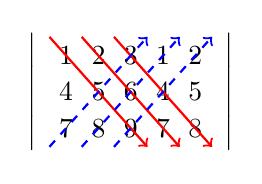
\begin{tikzpicture}
  \matrix (m) [matrix of math nodes, left delimiter=|, right delimiter=|] {
    1 & 2 & 3 & 1 & 2 \\
    4 & 5 & 6 & 4 & 5 \\
    7 & 8 & 9 & 7 & 8 \\
  };

  % Main diagonals (red solid lines -- positive terms)
  \draw[red, thick, ->] (m-1-1.north west) -- (m-3-3.south east);
  \draw[red, thick, ->] (m-1-2.north west) -- (m-3-4.south east);
  \draw[red, thick, ->] (m-1-3.north west) -- (m-3-5.south east);

  % Secondary diagonals (blue dashed lines -- negative terms)
  \draw[blue, thick, dashed, ->] (m-3-1.south west) -- (m-1-3.north east);
  \draw[blue, thick, dashed, ->] (m-3-2.south west) -- (m-1-4.north east);
  \draw[blue, thick, dashed, ->] (m-3-3.south west) -- (m-1-5.north east);
\end{tikzpicture}
\end{document}
